\toclesssection{Balanced Trees}

\toclesssubsection{Motivation}

\begin{frame}{Balanced Trees}{Motivation}
  \textbf{Binary search tree:}
  \begin{itemize}
  \item<2->
    With \texttt{\color{MainA}BinarySearchTree} we could perform an
    \texttt{\color{MainA}lookup} or \texttt{\color{MainA}insert}
    in {\color{MainA}$O(d)$}, with {\color{MainA}$d$} being the
    {\color{MainA}depth} of the tree
  \item<3->
    Best case: {\color{MainA}$d \in O(\log n)$}, keys are inserted randomly
  \item<4->
    Worst case: {\color{MainA}$d \in O(n)$}, keys are inserted in
    ascending / descending order {\color{MainA}$(20, 19, 18, \dotsc)$}
  \end{itemize}
\end{frame}

%-------------------------------------------------------------------------------

\begin{frame}{Balanced Trees}{Motivation}
  \textbf{Gnarley trees:}\hfill
  \onslide<2->
  \qrcode[height=5em]{\GnarleyTreesLink}\\
    \begin{itemize}
    \item \href{http://people.ksp.sk/~kuko/bak}{\color{blue}{\url{http://people.ksp.sk/~kuko/bak}}}
    \end{itemize}  
  \vspace{-2em}
  \begin{columns}
    \begin{column}[t]{0.5\linewidth}
      \onslide<3->
      \begin{figure}
        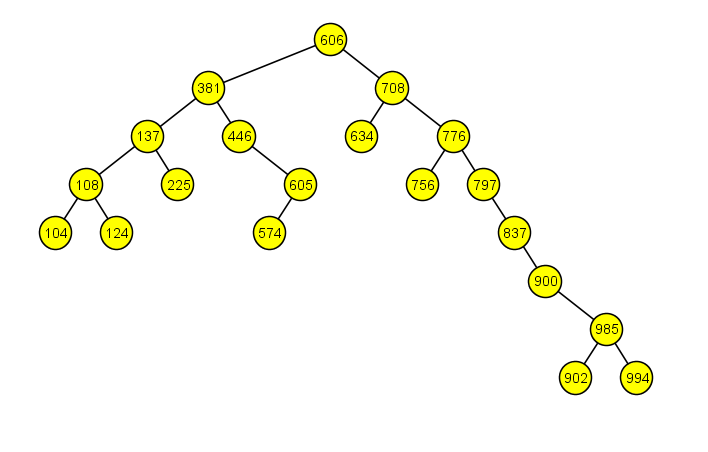
\includegraphics[width=\linewidth]{Images/Motivation/BinarySearchTree_Random.png}
        \caption{Binary search tree with random insert~\cite{gnarley_trees}}
        \label{fig:motivation:binary_search_tree_random}
      \end{figure}
    \end{column}
    \begin{column}[t]{0.5\linewidth}
      \onslide<4->
      \begin{figure}
        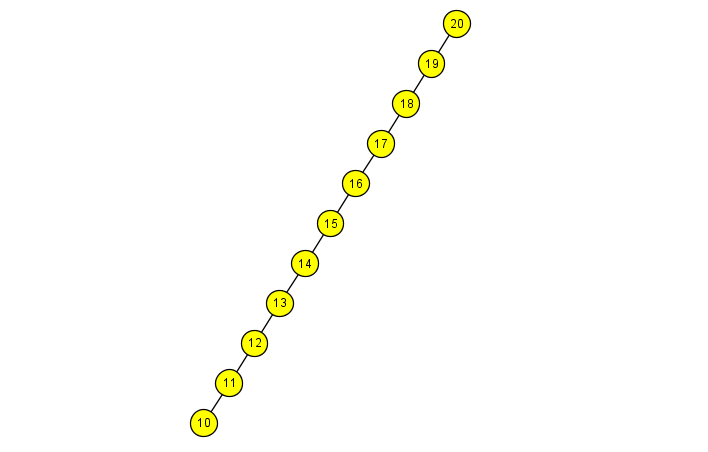
\includegraphics[width=\linewidth]{Images/Motivation/BinarySearchTree_Ordered.png}
        \caption{Binary search tree with descending insert~\cite{gnarley_trees}}
        \label{fig:motivation:binary_search_tree_ordered}
      \end{figure}
    \end{column}
  \end{columns}
 
\end{frame}

%-------------------------------------------------------------------------------

\begin{frame}{Balanced Trees}{Motivation}
  \textbf{Balanced trees:}
  \begin{itemize}
    \item<2->
      We do not want to rely on certain properties of our {\color{MainA}key set}
    \item<3->
      We explicitly want a depth of ${\color{MainA}O(\log n)}$
    \item<4->
      We {\color{MainA}rebalance} the tree from time to time
  \end{itemize}
\end{frame}

%-------------------------------------------------------------------------------

\begin{frame}{Balanced Trees}{Motivation}
  \textbf{How do we get a depth of {\color{MainA}$O(\log n)$}?}
  \begin{itemize}
    \item<2->
      \textbf{AVL-Tree:}
      \begin{itemize}
        \item<3->
          Binary tree with 2 children per node
        \item<4->
          Balancing via \enquote{\color{MainA}rotation}
      \end{itemize}
    \item<5->
      \textbf{(a,b)-Tree} or \textbf{B-Tree:}
      \begin{itemize}
        \item<6->
          Node has between ${\color{MainA}a}$ and ${\color{MainA}b}$ children
        \item<7->
          Balancing through {\color{MainA}splitting} and
          {\color{MainA}merging} nodes
        \item<8->
          Used in databases and file systems
      \end{itemize}
    \item<9->
      \textbf{Red-Black-Tree:}
      \begin{itemize}
        \item<10->
          Binary tree with \enquote{black} and \enquote{red} nodes
        \item<11->
          Balancing through \enquote{\color{MainA}rotation} and
          \enquote{\color{MainA}recoloring}
        \item<12->
          Can be interpreted as (2, 4)-tree
        \item<13->
          Used in C++ \texttt{std::map} and Java \texttt{SortedMap}
      \end{itemize}
  \end{itemize}
\end{frame}
